\chapter{Theory}

This thesis aims to enhance the runtime performance of ASP.NET Core applications by developing a route builder using C\# source generators. This approach, which involves generating static code, potentially leads to more efficient and scalable web applications.

In this chapter, we delve into the fundamental theories that underpin our work. It begins with an overview of various code generation techniques, outlining their advantages and disadvantages. This sets the stage for a more comprehensive understanding of the evolution of code generation in C\#, ultimately leading us to the advent and application of source generators. We then explore potential use cases of source generators and critically discuss their limitations, offering a balanced view of their practical implications.

Most importantly, this chapter presents a thorough literature review, which underscores the current body of research on code optimization, ASP.NET Core routing, and the performance implications of source generators. This review aims to identify gaps in existing research and draw attention to the potential contributions of this thesis. Through critical evaluation of the literature, we aim to highlight the significance of our work in this evolving field of study.

\section{Overview of Code Generation Techniques}

Code generation techniques encompass a range of strategies for creating code automatically or semi-automatically. These techniques can improve the development process by automating repetitive tasks, enhancing code quality, and optimizing performance. This section will explore the difference between runtime and static code generation. Both techniques will be discussed regarding its benefits and drawbacks, providing a comprehensive understanding of their applicability in different scenarios.

\subsection{Runtime Code Generation}

Runtime code generation, also known as dynamic code generation, is a technique where code is generated and executed during the runtime of a program. This approach enables developers to create code that adapts to the current execution context, allowing for more flexibility and customization. Runtime code generation can be employed in various scenarios, such as creating specialized implementations of algorithms or generating code based on user input or configuration data\cite{Chiba1995, Aycock2003}.

One standard method for achieving runtime code generation is Just-In-Time (JIT) compilation. JIT compilers translate portions of code, typically bytecode or intermediate language (IL) code, into machine code during the execution of a program\cite{Aycock2003}. This technique allows for optimizations based on the specific runtime environment, such as hardware characteristics or runtime data\cite{Gal2006}. The .NET runtime, for instance, employs a JIT compiler to compile the Common Intermediate Language (CIL) code into native code during the execution of a .NET application\cite{Esposito2014}.

Another approach to runtime code generation is to use reflection, a mechanism that allows a program to analyze and manipulate its structure and behavior during execution\cite{Maes1987}. In C\#, reflection can generate and invoke code dynamically, enabling developers to create, modify, and invoke types, methods, and properties at runtime\cite{Albahari2019}. While reflection provides a powerful and flexible means of generating code during runtime, it can introduce performance overhead due to the need to analyze and manipulate the metadata of the executing assembly\cite{Skeet2019}.

Using runtime code generation can offer several advantages, such as increased flexibility, adaptability, and the ability to perform optimizations based on runtime information\cite{Chiba1995, Aycock2003}. However, there are also potential drawbacks, including increased complexity, potential security risks, and performance overhead\cite{Aycock2003, Pobar2005}. In particular, the performance impact of runtime code generation is a significant concern when generating routes in an ASP.NET Core application. In addition, the use of reflection or JIT compilation may introduce latency or increased resource consumption during the execution of the application\cite{Pobar2005}.

\subsection{Static Code Generation}

Static code generation refers to generating code at compile time before the application is executed. This approach is in contrast to runtime code generation, which occurs during the execution of an application. With static code generation, the generated code is combined with the original source code during compilation, resulting in a single executable binary. This technique offers several advantages, including better performance, improved type safety, and easier debugging in some scenarios \cite{Chiba2000}.

Static code generation has been used to improve software performance and maintainability in various contexts. For instance, in web development, static site generators like Jekyll and Hugo produce HTML, CSS, and JavaScript files at build time rather than generating them on-the-fly for each request \cite{Biilmann2015}. This approach can improve performance and security, as a simple web server can serve the generated content without needing server-side processing.

One of the most common approaches to static code generation is metaprogramming, where code is generated or transformed by other code \cite{Cordy1992}. Various programming languages, including Lisp, Haskell, and C++, provide mechanisms for metaprogramming, such as macros, templates, or code generation tools. In the context of C\#, source generators are a relatively recent addition to the language that enables static code generation by analyzing the existing code and generating new source code during the compilation process \cite{Microsoft2022SourceGenerators}.

Static code generation can also be achieved using code generation tools and libraries. For example, tools like the Java Architecture for XML Binding (JAXB) and the .NET Framework's Windows Communication Foundation (WCF) generate code from XML schemas or interface definitions, respectively \cite{Vogel2023, Microsoft2021WhatLearn}. These tools help reduce the manual code developers must write and maintain, making keeping the codebase consistent with the underlying data structures or interfaces easier.

While static code generation offers numerous benefits, it also has some drawbacks. One of the main challenges is the increased complexity of the build process, as the code generation tools and libraries need to be integrated into the build pipeline. Additionally, the generated code may be less readable or harder to debug, as it may not directly correspond to the original source code or follow established coding conventions \cite{Chiba2000}.


\section{Evolution of C\# and Code Generation}

As C\# and the .NET ecosystem have evolved over the years, various code generation techniques have been developed and integrated into the platform. This section will discuss three significant milestones in the evolution of C\# code generation: T4 templates, the Roslyn API, and the introduction of Source Generators. Each milestone represents a step forward in how developers can generate and manipulate code in C\# applications, providing more efficient and sophisticated methods for managing complex projects. Understanding the context and limitations of each technique is essential for appreciating the current state of code generation in C\# and the role of Source Generators in addressing the challenges of previous approaches.

\subsection{T4 Templates and their Limitations}

Text Template Transformation Toolkit (T4) is a code generation technology that has been a part of the .NET ecosystem since the release of Visual Studio 2005. T4 templates are text-based templates that allow developers to generate code using a mixture of static text, control logic, and data from external sources \cite{Klein2010}. T4 has been widely used in various scenarios, including generating code for data access layers, model-driven development, and code scaffolding \cite{Vogel2010}.

However, T4 templates have certain limitations that can make them less suitable for certain code-generation tasks. One of the primary drawbacks of T4 templates is that they lack a real-time execution. This means that the T4 templates only transform when you save the template file or when you manually initiate the transformation. They do not automatically update when the data they depend on changes, which can lead to outdated output \cite{Klein2010}. Furthermore, T4 templates do not provide any means to validate the generated code during the generation process, which can lead to syntax errors or other issues in the generated code that may not be detected until the code is compiled \cite{Vogel2010}.

Another limitation of T4 templates is that they do not support direct unit testing. Since the templates are not C\# Code, they can not be tested with the same unit testing framework as the rest of the project. Instead, one would have to transform the templates and test the outcome. Additionally, one of the biggest drawbacks of T4 templates is the lack of a robust mechanism for integrating with the C\# language features and the compiler, which can make it difficult to achieve advanced code generation scenarios or leverage the full power of the C\# language in generated code \cite{Esposito2014}.

These limitations have led to the exploration of alternative code generation techniques within the C\# and .NET communities, with the Roslyn API and Source Generators emerging as more advanced and flexible solutions for code generation tasks.

\subsection{Roslyn API}

The Roslyn API, introduced by Microsoft in 2011, is a set of open-source compilers and code analysis APIs for C\# and Visual Basic .NET (VB.NET) languages \cite{CSharpRoslyn}. Roslyn's primary goal is to enable developers to write custom tools and analyzers, providing a deep understanding of the source code by exposing its syntax trees, symbols, and semantic information \cite{Vermeir2022}. The API is designed to be language- and platform-agnostic, which makes it suitable for various use cases, such as code analysis, refactoring, and code generation \cite{Vermeir2022}.

One of Roslyn's significant advantages is its ability to perform real-time code analysis. This feature allows developers to identify potential issues and opportunities for refactoring as they write code, significantly reducing the time spent on manual code reviews \cite{Vermeir2022}. Furthermore, Roslyn provides a platform for developers to create custom diagnostics and refactorings, which can be easily integrated into IDEs like Visual Studio, enabling a more streamlined development process \cite{CSharpRoslyn}.

Although Roslyn offers many benefits over T4 templates, it also has its limitations. While Roslyn is excellent for code analysis and refactoring, it is not specifically designed for code generation like T4 templates \cite{Vermeir2022}. However, with the introduction of source generators in C\# 9, this gap has been addressed, allowing developers to leverage the power of Roslyn for code generation tasks as well \cite{Carter2020}.

\subsection{Introudction of Source Generators}

The introduction of source generators in C\# 9 offers developers a novel method for executing compile-time code generation in .NET applications, thus overcoming the limitations associated with runtime code generation and T4 templates \cite{Torgersen2020}. As shown in Figure \ref{fig:source_generators_workflow}, source generators operate as part of the normal compilation process.

\begin{figure}[H]
\centering
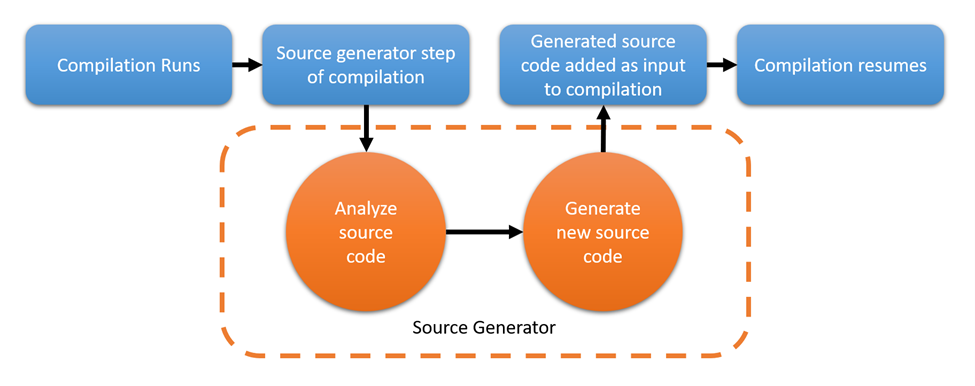
\includegraphics[width=0.8\textwidth]{graphics/source-generator-visualization.png}
\caption{Source Generators Overview}
\label{fig:source_generators_workflow}
\end{figure}

The figure above illustrates the integration of source generators in the C\# compilation process. It commences with the running of the compilation, which then transitions to the source generator step. This segment involves two key operations: "Analyze source code" and "Generate new source code." The analyzed code provides important information that the source generators employ to produce new source code. Once the source generator completes these tasks, the generated source code is added back as input to the compilation process. Following this addition, the compilation process resumes, thus concluding the sequence.

Through the Roslyn API, source generators can interface with the abstract syntax tree (AST) and the semantic model of the code being compiled. This capability enables them to generate code that harmonizes with the original source \cite{CSharpRoslyn}. The resultant integration fosters seamless interaction between the generated and the handwritten code, and it also allows for the enforcement of type safety and other compile-time checks \cite{Carter2020}. This integration and safety considerably enhance the developer experience in code generation within the .NET ecosystem.

Source generators also pioneer new prospects for code optimization and performance improvements. By generating code during compile-time, source generators can reduce the need for resource-demanding runtime operations, thus providing a more performance-efficient alternative for code generation tasks \cite{CSharpRoslyn}.

The emergence of source generators has stimulated innovation and encouraged the development of new tools and libraries in the .NET ecosystem. Developers' growing adoption of source generators is leading to the creation of an increasing number of libraries and tools that facilitate and simplify the code generation process. This flourishing ecosystem underscores the utility of source generators in contemporary .NET development, granting developers a potent, performant, and user-friendly mechanism for generating code at compile-time.

\section{Use Cases and Applications of Source Generators}

As the C\# language and .NET platform have evolved over time, the emergence of source generators has opened up new opportunities for developers to enhance their applications' performance, maintainability, and robustness. Source generators can be applied to various aspects of software development, including, but not limited to, serialization, logging, dependency injection, and ASP.NET Core routing. This section aims to explore the specific use cases and applications of source generators, examining the current approaches and their limitations, as well as the potential opportunities for improvement that source generators provide.

In the following subsections, we will delve into each of the aforementioned use cases, discussing their significance, existing implementations, and challenges. We will also investigate how source generators can be leveraged to optimize these areas of software development. While this section covers various possible applications of source generators, the primary focus of this thesis will be on ASP.NET Core routing. By examining the current approaches and limitations in this area and the potential opportunities for improvement that source generators provide, we aim to demonstrate their effectiveness and practicality in enhancing the performance of ASP.NET Core applications.

\subsection{Serialization}

Serialization is the process of converting an object's state into a format that can be stored, transmitted, and reconstructed later \cite{Fowler2002}. In the .NET ecosystem, serialization is essential for various tasks, such as data persistence, remote procedure calls, and message-passing systems \cite{Fowler2002}. Several serialization libraries are available for .NET, such as XmlSerializer, DataContractSerializer, and Newtonsoft.Json, each offering different levels of flexibility and performance.

One of the challenges in serialization is achieving high performance, especially when dealing with large datasets or performance-critical applications. Traditional serialization libraries often rely on reflection to inspect and manipulate object data at runtime, which can introduce significant overhead and negatively impact the application's performance \cite{NewtonsoftJsonPerformance}. Source generators offer a potential solution to this issue by enabling the generation of serialization code at compile-time, thereby eliminating the need for runtime reflection.

Using source generators for serialization has several advantages. First, it allows for the generation of efficient and optimized serialization code tailored to the specific types being serialized \cite{CSharpRoslyn}. This can result in significant performance improvements compared to using generic runtime-based serializers, which need to handle a wide variety of data types and scenarios \cite{NewtonsoftJsonPerformance}. Second, generating serialization code at compile-time can help identify potential issues, such as missing or incompatible attributes, before the application is deployed, leading to a more robust and reliable serialization process.

Several libraries have started leveraging source generators to provide high-performance serialization in .NET. One such library is System.Text.Json, which is a built-in JSON serialization library in .NET Core 3.0 and later versions \cite{SystemTextJson}. Since .NET 6, System.Text.Json can use source generators to generate custom serialization code for specific types at compile-time, offering significant performance improvements compared to its runtime-based counterparts \cite{SystemTextJsonSourceGen}. By embracing source generators, serialization libraries can deliver more efficient, reliable, and performant solutions to .NET developers.

\subsection{Logging}

Logging is an essential aspect of software development, as it allows developers to monitor, diagnose, and analyze the behavior of their applications \cite{Fowler2002}. Several popular logging libraries exist for .NET, such as log4net, NLog, and Serilog, each with its own set of features and performance characteristics \cite{LoggingDotnet}. However, logging can introduce overhead during runtime, as log entries need to be formatted, filtered, and written to various output targets, such as files, databases, or external services \cite{Serilog}.

Source generators have the potential to enhance the performance and capabilities of logging libraries by generating code at compile-time instead of performing string interpolation, method calls, and other costly operations at runtime \cite{CSharpRoslyn}. By generating specialized code for specific logging scenarios, source generators can reduce the amount of runtime overhead associated with logging, leading to improved application performance \cite{Carter2020}. Additionally, source generators can analyze the logging code during compilation to identify potential issues, such as incorrect log levels or formatting, and provide developers with feedback through compiler warnings or errors \cite{Torgersen2020}.

The use of source generators for logging can also simplify the process of configuring and setting up logging libraries. By analyzing the application code and configuration, source generators can generate tailored logging implementations specific to the application's requirements, eliminating the need for manual configuration or complex initialization code \cite{CSharpRoslyn}. This approach can lead to cleaner, more maintainable code and a more streamlined development experience.

\subsection{Dependency Injection}

Dependency Injection (DI) is a widely-used design pattern that promotes loosely-coupled and modular software design by injecting dependencies into an object instead of having the object create them directly \cite{Martin2003}. In the .NET ecosystem, the built-in DI container and various third-party libraries, such as Autofac and Ninject, facilitate dependency injection \cite{DIContainers}. However, dependency resolution at runtime can introduce overhead, as the DI container needs to manage and resolve dependencies, potentially affecting application performance \cite{Blumhardt2010}.

Source generators offer an opportunity to optimize the DI process by generating code for dependency resolution at compile-time \cite{CSharpRoslyn}. By analyzing the application's codebase and identifying the required dependencies, source generators can create tailored code to resolve and manage dependencies, effectively eliminating the runtime overhead associated with dependency resolution \cite{Carter2020}. The generated code can also benefit from advanced compiler optimizations, further enhancing the performance of the DI process \cite{Torgersen2020}.

Additionally, source generators can help enforce best practices in DI configuration by analyzing the code and providing compile-time feedback on potential issues, such as missing or incorrect registrations \cite{CSharpRoslyn}. This can lead to more robust and maintainable applications by ensuring that dependency injection is correctly configured and implemented.

\subsection{ASP.NET Core Routing}

ASP.NET Core Routing is a critical component of web applications built on the ASP.NET Core framework, responsible for mapping incoming requests to the appropriate actions in controllers \cite{Microsoft2023RoutingCore}. The routing system uses a combination of route templates, constraints, and conventions to determine the best match for incoming requests \cite{Microsoft2023RoutingCore}. While the built-in routing system is highly customizable and extensible, it relies on runtime reflection to discover and invoke the appropriate action methods, which can introduce performance overhead \cite{Microsoft2023RoutingCore}.

The introduction of source generators in C\# 9 presents an opportunity to optimize the routing process by generating code at compile-time for route resolution and action invocation \cite{CSharpRoslyn}. By analyzing the application's codebase and extracting routing information from controller actions and route attributes, source generators can generate efficient and optimized code for routing, eliminating the need for runtime reflection \cite{Carter2020}. This can lead to significant performance improvements, especially in scenarios with a large number of routes or high request loads \cite{Slimak2022}.

Moreover, source generators can enhance the developer experience by providing compile-time feedback on potential routing issues, such as conflicting routes or incorrect route templates \cite{CSharpRoslyn}. This can help developers catch and fix routing problems early in development, leading to more robust and maintainable web applications.

\section{Limitations and Challenges of Source Generators}

While introducing source generators in C\# 9 has brought about significant advancements in code generation, it is important to recognize that they also come with limitations.

Firstly, source generators do not modify existing code; they only add new code to the compilation. This means that developers cannot use source generators to automatically refactor or change the behavior of existing code \cite{CSharpRoslyn}. While this restriction is intended to prevent unexpected side effects and maintain the integrity of the original source code, it can limit the scope of applications for source generators \cite{Carter2020}.

Secondly, source generators are executed during the compilation process; hence, their runtime is included in the overall compile time of the application \cite{CSharpRoslyn}. As a result, poorly optimized source generators can significantly increase compile times, affecting the developer experience, particularly in large codebases \cite{Carter2020}.

Furthermore, source generators work on a syntax tree representation of the code, meaning that they do not have access to the results of previous compiler phases, such as constant folding or definite assignment analysis \cite{Torgersen2020}. This can make certain code generation tasks more complex or even impossible in some cases \cite{CSharpRoslyn}.

Lastly, while source generators have the potential to significantly improve the performance of applications by moving computation from runtime to compile-time, they also require developers to think in a new paradigm. This could potentially increase the complexity of the code and require a learning curve for developers new to the concept of metaprogramming \cite{CSharpRoslyn}.

\section{Relevant Academic Literature and Research}

Performance optimization is a crucial aspect of computer science, with numerous studies exploring its significance and potential areas of enhancement. This section provides a literature review on topics pivotal to this thesis - code generation and optimization, the impact of reflection on performance, the challenges in ASP.NET Core routing, and the current state of research regarding source generators. This exploration of the existing academic literature will identify gaps in current research and pave the way for the original contributions of this bachelor's thesis.

\subsection{Code Generation and Optimization}

Code generation and optimization, being essential areas of research within computer science, have the power to augment system performance, reduce memory usage, and boost overall efficiency.

Early studies in this field primarily focused on compiler optimizations. Aho et al. \cite{Aho2007} offer a thorough study of various optimization techniques employed in modern compilers, such as constant folding, dead code elimination, and loop optimizations. Their work underscores the importance of these methods in enhancing the speed of compiled programs.

As the field has evolved, research has branched out to examine dynamic code generation and optimization. Kistler and Franz \cite{Kistler2003} put forward a system that generates code at load-time and continuously optimizes it at run-time. This approach allows software to adjust to the exact hardware capabilities at the time of execution, thereby overcoming modularization overheads through global optimization. Furthermore, it enables software to adapt to changing user behavior and incorporate dynamic link libraries at a later stage. While they caution that the cost-benefit ratio of continuous optimization can vary, it can lead to speed-ups of more than 120\% under ideal conditions. This indicates the significant potential of dynamic code generation and optimization when applied correctly.

In recent times, machine learning has started to play a significant role in compiler optimization. Madhav, Singaravel, and Karmel \cite{Shreyas2021} discuss how compiler optimization techniques contribute to efficient computing by enabling developers to maximize hardware performance without significant cost implications. Of particular interest in their study is the prospect of machine learning revolutionizing compiler optimization, leading to a more sustainable and efficient computing experience for both developers and users.

The code generation and optimization field continues to evolve with new techniques and technologies, promising further advancements and discoveries. This section sets the stage for exploring how these developments can be harnessed in the context of source generators and performance optimization.

\subsection{Reflection Usage and Performance Implications}

Reflection is a mechanism that allows programs to inspect and manipulate their own structure and behavior at runtime. While this capability can be highly beneficial, it also carries with it performance considerations.

Reflection operations necessitate the dynamic resolution of types, which requires the Common Language Runtime (CLR) in .NET (or equivalent in other languages) to load classes and information at runtime. This contrasts with non-reflective code, which loads classes and information at compile time. As a result, reflective operations tend to have slower performance than non-reflective ones due to the additional overhead required for dynamic resolution. An extensive study by Tudose et. al. \cite{Tudose2013} states that reflective operations are time-consuming, and developers should avoid frequently calling them if possible due to their performance overhead.

Despite these performance considerations, reflection remains a significant technique widely used across various programming ecosystems due to its flexibility and adaptability. Specifically, in the .NET ecosystem, an investigation revealed that over 15\% of more than 6 million NuGets utilize reflective techniques \cite{Beaumont2022}. This widespread usage underscores reflection's inherent value and versatility in software development, even in the face of potential performance costs.

This dichotomy—reflection's widespread use and the associated performance penalties—highlights the necessity for alternative strategies. The pursuit of mechanisms that can provide reflection-like flexibility with more optimal performance characteristics is gaining importance.

The study \cite{Beaumont2022} emphasizes that understanding and employing reflection techniques are valuable for developers at all stages of their careers, yet also cautions about potential performance implications. This reality underscores the need for performant alternatives that can support the significant portion of NuGets relying on reflection, thereby potentially enhancing their performance while retaining their functionality.

Recognizing this need, the field is undergoing a shift towards more efficient approaches, paving the way for exciting possibilities in software optimization and performance improvement. This evolution calls for continuous research and innovation, aiming to strike a balance between flexibility and efficiency in code generation and execution. In the following sections, we will first look at the performance issues in ASP.NET Core routing, particularly related to its use of reflection. Finally, we will discuss how source generators can provide a solution to these problems, showing how they can improve performance while retaining the benefits of reflection.

\subsection{Performance Implications of ASP.NET Core Routing Mechanisms}

ASP.NET Core is a renowned technology for building web applications and APIs. Its appeal among developers is largely influenced by its performance attributes - execution speed, delivery time, and startup time.

A comparison study by Kronis and Uhanova \cite{Kronis2018} delved into the performance characteristics of ASP.NET Core and Java EE. They created benchmarks as REST services that processed data in JSON format and ran these benchmarks on the Kestrel web server. Although their investigation did not directly address startup time, it provided valuable insights into the relative performance capabilities of these two platforms.

Karlsson \cite{Karlsson2021} took a slightly different approach, pitting ASP.NET Core and Express.js against each other, with both being used alongside a MySQL database to construct Web APIs. Karlsson's findings revealed that, in the context of a RESTful API, ASP.NET Core handled lower loads more efficiently, but Express.js had the upper hand when processing a larger volume of concurrent requests. Interestingly, with the new querying language GraphQL, Express.js either equaled or surpassed ASP.NET Core in terms of response times and resource usage.

Even with such extensive studies, the performance implications of the routing mechanism, a crucial determinant of the startup time for ASP.NET Core applications, have received less scrutiny. The route builder in ASP.NET Core, which utilizes reflection to map controllers and actions to routes, might be a performance pinch point due to the known performance overheads associated with reflection. Thus, optimizing this routing mechanism to lessen the dependency on reflection and potentially improve startup time merits investigation.

These studies provide an insightful comparison of ASP.NET Core's performance with other technologies, but they also highlight a demand for more granular research on ASP.NET Core-specific aspects, such as routing mechanism and startup time. Such focus could reveal new ways to optimize these aspects and enhance application performance. In the following section, we will delve into this untapped potential, exploring possible avenues for performance improvement.

\subsection{Source Generators and Performance Improvements}

In the relatively uncharted domain of Source Generators in C\#, Slimak's work \cite{Slimak2022} stands out. His thesis offers an in-depth guide to Source Generators, a .NET feature with significant potential to enhance various aspects of software development, such as performance and development time. The thesis aims to help readers understand Source Generators, their purpose and use cases, and how they differentiate from other prevalent code generation options in C\#. The work further explores the use of Source Generators in enterprise applications and proposes a more complex framework that could generate common boilerplate code, thus improving development efficiency. However, the thesis underscores the current immaturity of Source Generators and the challenges they pose for integration into existing .NET tools, like Visual Studio and IntelliSense.

Supplementing the insights from Slimak's research, another study worth discussing is Franz's \cite{Franz2022}, entitled "Trends im Compilerbau". Though written in German, the paper provides a wider view on the trends shaping the field of compiler construction, with a particular focus on Source Generators and Just-In-Time Compilers. Using a dataset from the IEEE Xplore library, Franz emphasizes how active and vibrant the compiler construction research field remains, even with its considerable history. The emergence of new tools, like source generators, is sparking fresh inquiries. A key takeaway from Franz's study is the sustained focus on code optimizations—these efforts to enhance the output performance of compilers remain a primary concern in both practical and research contexts.

Adding to these scholarly resources, the book "Introducing .NET 6" by Nico Vermeir \cite{Vermeir2022} offers a practical perspective. Though not a research paper, the book contains a chapter titled ".NET Compiler Platform" that explains Source Generators among other topics. Vermeir describes how the .NET Compiler Platform, previously known as project Roslyn, provides strength and flexibility to .NET. Additionally, the author discusses source generators, highlighting how they leverage Roslyn to generate code at compile time and incorporate that generated code into the compilation process.

\section{Critical Evaluation of the Literature}

This section critically analyzes the strengths and weaknesses of existing research regarding Source Generators, reflection, ASP.NET Core routing mechanisms, and code generation and optimization. Additionally, gaps and inconsistencies in the literature are pointed out.

\subsection{Strengths and Weaknesses of the Existing Research}

The current literature on the topics of interest exhibits a variety of strengths. It thoroughly examines the areas of code generation and optimization, demonstrating how these fields have evolved from early compiler optimizations \cite{Aho2007} to dynamic code generation techniques \cite{Kistler2003}, and even the application of machine learning \cite{Shreyas2021}. This wealth of research serves as a solid foundation for understanding the optimization landscape and preparing for its future.

Similarly, the analysis of reflection's performance implications and the extensive use of reflective techniques, despite their overhead, is well covered \cite{Tudose2013, Beaumont2022}. It provides a comprehensive understanding of the trade-offs and opportunities involved in using reflection in software development.

A major strength of Slimak's thesis \cite{Slimak2022} is its practical focus on how Source Generators can be employed in real-world applications. Simultaneously, Franz's paper \cite{Franz2022} broadens the perspective by analyzing ongoing trends in compiler construction, underscoring this field's vibrant and active state.

However, the literature also has some limitations. Although machine learning's role in compiler optimization is briefly touched on by Madhav, Singaravel, and Karmel \cite{Shreyas2021}, a more in-depth exploration of this intersection is lacking. Additionally, while the impact of reflection on performance has been discussed, there's scant literature on alternatives that maintain reflection's versatility without its performance cost.

Regarding ASP.NET Core, studies like those by Kronis and Uhanova \cite{Kronis2018} and Karlsson \cite{Karlsson2021} provide a comparison of its performance with other technologies, but they do not specifically address the performance implications of the routing mechanism, which is a crucial determinant of startup time for ASP.NET Core applications.

\subsection{Gaps or Inconsistencies in the Literature}

While the existing research provides valuable insights, several gaps and potential inconsistencies need to be addressed.

There is a significant gap in research concerning the performance implications of ASP.NET Core's routing mechanisms. While there are comparative studies of ASP.NET Core's performance against other frameworks, there's a dearth of focused examination on its internal aspects such as routing mechanism performance and startup time optimization.

Additionally, although Slimak's work on Source Generators \cite{Slimak2022} is comprehensive, it also emphasizes the immaturity of Source Generators and their integration challenges with existing .NET tools. This highlights the need for more research to make Source Generators more accessible and mature.

Another crucial gap is the lack of extensive research into alternatives to reflection that maintain its versatility while reducing performance costs. Despite its performance overhead, the widespread use of reflection represents a significant opportunity for future research.

In terms of inconsistencies, there seems to be a lack of consensus on the best use cases for dynamic code generation and optimization techniques. For instance, Kistler and Franz \cite{Kistler2003} suggest that continuous optimization can lead to significant speed-ups, but they also note that the cost-benefit ratio can vary. This indicates the need for further exploration to determine the specific conditions under which these techniques are most effective.

\section{Contribution of this thesis}

This thesis contributes to the current body of knowledge in several distinct ways, bridging existing gaps and enhancing our understanding of critical issues pertaining to code generation, optimization, and performance improvement in software development.

Firstly, this research expands on the application of Source Generators in the .NET ecosystem, primarily focusing on performance optimization. Despite the promising potential of Source Generators, previous research indicates that this technology is currently in a state of relative immaturity \cite{Slimak2022}. This thesis contributes a systematic analysis of Source Generators, evaluating their strengths, weaknesses, and areas of application in the context of software performance improvement.

Secondly, this thesis critically investigates the impact of ASP.NET Core's routing mechanisms on performance—a subject that has received limited attention in the existing literature. By thoroughly examining routing mechanisms and their relationship to startup time, the study uncovers new ways to enhance the performance of ASP.NET Core applications.

Lastly, with respect to reflection, existing research has highlighted its associated performance overhead. This study delves into a practical approach to alleviate these performance implications without forsaking the benefits of reflection. Rather than seeking alternatives to reflection, the study attempts to reduce the need for reflection at runtime, thereby preserving its functionality and versatility.